\documentclass[10pt]{article}
\usepackage[a4paper,top=.8in,bottom=.77in,left=.88in,right=.88in]{geometry}
\usepackage{amsmath,amssymb,graphicx,booktabs,xcolor,hyperref,fancyhdr}
\definecolor{ink}{RGB}{30,59,72}\definecolor{teal}{RGB}{17,108,108}\definecolor{muted}{RGB}{65,86,94}
\hypersetup{colorlinks=true,urlcolor=teal,linkcolor=teal,pdftitle={Eight boundary points beyond the four-period ring}}
\pagestyle{fancy}\fancyhf{}\renewcommand{\headrulewidth}{0pt}\renewcommand{\footrulewidth}{.3pt}\fancyfoot[L]{\footnotesize\sffamily\color{muted} NO-THREE-IN-LINE \enspace / \enspace CONSTRUCTION NOTE}\fancyfoot[R]{\footnotesize\sffamily\thepage}
\setlength{\parindent}{0pt}\setlength{\parskip}{5pt}
\newcommand{\head}[1]{\par\vspace{4pt}{\Large\sffamily\bfseries\color{ink}#1}\par}
\newcommand{\sub}[1]{\par\vspace{3pt}{\large\sffamily\bfseries\color{ink}#1}\par}
\newcommand{\eyebrow}[1]{{\small\sffamily\bfseries\color{teal}#1}\par}
\newcommand{\file}[1]{\texttt{\detokenize{#1}}}\newcommand{\F}{\mathbb F_p}\newcommand{\e}{\varepsilon}
\newcommand{\qed}{\hfill$\square$}
\begin{document}
\eyebrow{DISCRETE GEOMETRY \quad / \quad RESEARCH NOTE \hfill 19 NOVEMBER 2026}
\vspace{3pt}{\LARGE\sffamily\bfseries\color{ink}Eight boundary points beyond the four-period ring}\par
Let $F(n)$ be the largest size of a set in $\{0,\ldots,n-1\}^2$ with no three distinct points on an ordinary straight line. Write $F_{1/2}(n)$ when the set must also be invariant under the board's half-turn $(x,y)\mapsto(n-1-x,n-1-y)$.
\sub{An infinite family strictly above $3n/2$}
\textbf{Theorem A.} For every prime $p\equiv1\pmod{24}$, there is an explicit half-turn invariant set of $6p+2$ points on a board of side $n=4p+1$. In particular,
\[
 F(n)\ \ge\ F_{1/2}(n)\ \ge\ \frac{3n+1}{2}\qquad(n=4p+1,\ p\equiv1\!\pmod{24}).
\]
The construction retains all $6(p-1)$ points of a known modular ring [3] and adds eight. Its gain over $3n/2$ is \emph{exactly $1/2$, not a positive multiple of $n$}. An elementary, computer-free version works for \emph{every} prime $p\equiv1\pmod{840}$, with any nonsquare level. The broader progression has an analytic proof for $p>50625$ and explicit finite certificates below that cutoff.
\begin{center}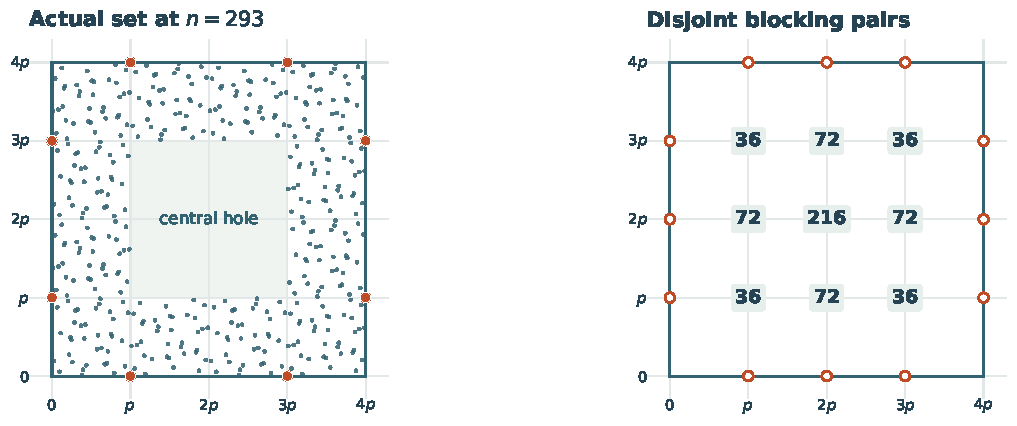
\includegraphics[width=.85\linewidth]{ring-figure.pdf}\end{center}
{\small Left: all 432 old points and eight new boundary points for $p=73$. Right: the number of disjoint, centrally opposite pairs of old points about each \emph{interior coarse site}; each such pair blocks inserting that site. All twelve open-side sites (circles) are individually protected at the selected level.}
\sub{A rule for arbitrary sides}
\textbf{Theorem B.} If $p>3$ is prime and $3p\le n\le4p$, a half-turn invariant construction gives
\[
 F_{1/2}(n)\ \ge\ 2n-2p-42.
\]
At $p\equiv1\pmod{12}$ the construction has at least $2n-2p-6$ points. The generator accepts \emph{every} positive integer $n$. Taking the first prime $p\ge n/4$ for large $n$ gives $F_{1/2}(n)\ge(3/2-o(1))n$ by the prime number theorem. The unrestricted coefficient $3/2$ is classical [1,2]; this is not a proof of a larger coefficient. The point of the rectangular rule is that it needs no prime progression and can use a prime \emph{above} $n/4$, not just embed a smaller square.

\sub{Which lower bound improves?}
On an infinite sequence, the anchored family crosses the line $3n/2$ by a constant. On certain intervals it also beats the simple rule ``embed the classical frame at the largest prime below $n/2$'' by a number of points growing at least logarithmically in the side (Corollary C). These are different comparisons. For example, the construction gives 1500344 points at $n=1000229$: its surplus over $3n/2$ is $1/2$, not a growing density increment.

\newpage\eyebrow{01 \quad / \quad PROTECTING THE BOUNDARY}
\head{Why the eight points do not make a triple}
Take an odd prime $p\equiv1\pmod{24}$, a nonsquare $k\in\F^*$ and the board $[0,4p]^2\cap\mathbb Z^2$. Let $\chi$ denote the quadratic character and let $e(u)=0$ for a square, $1$ for a nonsquare. The old set $O$ consists of sites $(x,y)$ such that
\[
 xy\equiv k\pmod p,\quad (x+y)\bmod2=e(x\bmod p),\quad
 (\lfloor x/p\rfloor,\lfloor y/p\rfloor)\notin\{1,2\}^2.
\]
The residue prevents either coordinate being a multiple of $p$. A fibre is the set of lifts of one residue $(u,k/u)$. It has six old points: in the $4\times4$ sheet square, take one checkerboard half of the twelve outer cells. These are the masks of [3]. They have no three in line; their nonaxis primitive directions are $(1,\pm1),(1,\pm3),(3,\pm1)$ up to sign. The $4\times4$ lists on page 4 also give a direct finite check.

\textbf{Old triples.} Reduction of a primitive integer line is a genuine line over $\F$; it meets $xy=k$ in at most two residues. In an old triple two points would be in the same fibre. An axis through them cannot meet another fibre. In a nonaxis primitive direction $(a,b)$ their possible other fibre has first coordinate
\[
 u'=-ak/(bu),
\]
by the product of the two roots of the line--hyperbola equation. Here $-a/b$ is a square since $-1,3$ are squares. Thus $e(u')=1-e(u)$. But physical parity $x+y\bmod2$ is constant on an integer line of odd--odd primitive direction. This rules out the third point. The entire ring is half-turn invariant: $u\mapsto-u$ preserves $e(u)$, and the outer cells and physical parity are preserved.

\textbf{Coarse anchors.} Select two out of the three noncorner coarse sites on each side of $p\{0,1,2,3,4\}^2$. There are $3^4=81$ choices. For instance use the orbit of $(0,p)$ under the eight square symmetries: on each side select indices 1 and 3. The anchors alone form a cap: a non-edge line meets the boundary of a convex square in at most two points; each edge gets two. A primitive nonaxis line through two coarse sites has height $H=\max(|a|,|b|)\le4$. Its carrier points would have to satisfy $ab\,t^2=k\pmod p$. The signed factors of $ab$ are built from $-1,2,3$, all squares. So it misses the carrier. The same is true of coarse axis lines.

\textbf{One anchor, two old points.} Fix an open-side coarse site $q$. Every entering nonaxis line has only \emph{one} ray inside the board, parametrized $q+t(a,b)$ for positive integers $t\le4p/H$. The carrier equation is again $ab\,t^2=k\pmod p$. When $H\le4$ there is no root. When $H\ge8$, $t\le p/2$, so a root pair $r,-r\bmod p$ contributes at most one integer (and if $p\mid ab$ there are no roots). It remains to check $5\le H\le7$. Below we choose $k$ so that any roots have least absolute representative $r$ satisfying
\[
 0<r<(1-4/H)p.
\]
Then $t<p$ and $p-r>4p/H$, so the ray again has at most one point. Only odd--odd directions need be considered: for even--odd directions in this height range, $t<p$ and the roots $t,p-t$ have opposite parity. The $x$-residues are negatives so have the same character, whereas physical parity differs because $a+b$ is odd. Hence at most one root point belongs to $O$. This argument covers all slopes, including those much larger than $p$.

\newpage\eyebrow{02 \quad / \quad SELECTING THE LEVEL}
\head{A finite list of root inequalities}
\textbf{A short proof on a subprogression.} For every prime $p\equiv1\pmod{840}$, quadratic reciprocity makes $-1,2,3,5,7$ squares. Every signed nonzero product $ab$ with $H\le7$ is then a square; $k$ is not. There are no small-height roots at all. The previous page proves Theorem A on this progression without computation or tuning. Infinitely many such primes exist by Dirichlet's theorem.

\textbf{The full progression.} At $p\equiv1\pmod{24}$, only $5,7$ can introduce a nonsquare in the odd--odd cases $5\le H\le7$. The possible nonsquare products are among
\[
 \begin{array}{ll}H=5:&d=\pm5,\ \pm15,\\H=7:&d=\pm7,\ \pm21,\ \pm35.\end{array}
\]
Discard the squares. For a fixed nonsquare $\nu$, take a root $s_d^2=\nu/d\pmod p$ for each retained $d$. Set $b_d=5$ at height 5 and $b_d=3$ at height 7, and $B=\prod_d b_d$. Partition the unit cube into $B$ boxes with these coordinate subdivisions. The $B+1$ fractional-part vectors $(\{j s_d/p\})_d$, $0\le j\le B$, give two in one box. Their index difference $1\le z\le B$ satisfies $\|zs_d/p\|<1/b_d$ simultaneously. If $p>B$, $z\neq0\pmod p$. Take $k=\nu z^2$. The least roots at height 5 are then $<p/5$, and those at height 7 are $<p/3<3p/7$, as required. If the product list is empty just take $k=\nu$.

If 5 and 7 are both nonsquares, $B=5^4 3^4=50625$ because 35 is square. If only 5 is nonsquare then $B=5^4 3^2=5625$; if only 7 is nonsquare then $B=3^6=729$; otherwise $B=1$. Thus $p>50625$ suffices in all cases.

\textbf{Finite verification.} Among primes $p\equiv1\pmod{24}$ with $p\le B(p)$, there are exactly 194. The accompanying CSV gives a nonsquare $k$ for every one. For 191 rows, computing the least roots of $k/d$ verifies $Hr<(H-4)p$ directly. For the remaining $(p,k)=(73,28),(97,17),(193,20)$, the independently written checker enumerates $O$ from the defining congruence and checks \emph{all} directions from each of the twelve open-side sites against $O$, as well as every pair-anchor line. These finite checks use integer arithmetic only; see \file{code/check_certificates.py}. This completes Theorem A.\qed

\sub{Examples}
\begin{center}\begin{tabular}{rrrrr}\toprule
Prime $p$ & Level $k$ & Side $4p+1$ & $|O|$ & With eight anchors\\\midrule
73 & 28 & 293 & 432 & 440\\97 & 17 & 389 & 576 & 584\\1009 & 11 & 4037 & 6048 & 6056\\2521 & 11 & 10085 & 15120 & 15128\\250057 & 5445 & 1000229 & 1500336 & 1500344\\\bottomrule\end{tabular}\end{center}
\small The first four coordinate files were independently checked at every point against every other point by equality of normalized unoriented integer directions. The last row is a parameter-only example certified by the arithmetic criterion. These are not claims of finite records. The initial ring is not claimed new; neither [1] nor the statement of [3] includes these protected off-carrier boundary sets. No exhaustive priority claim is made.

\newpage\eyebrow{03 \quad / \quad ARBITRARY SIDE LENGTHS}
\head{Rectangular masks instead of cropping a square}
Let $p>3$, $3p\le n\le4p$, and choose $c$ nonsquare if $p\equiv1\pmod{12}$, otherwise put $c=1$. Let $2\alpha=n-1\pmod p$. Use the translated residues $(\alpha+u,\alpha+c/u)$, $u\ne0$. The board's half-turn pairs fibre $u$ with fibre $-u$. With $(x_0,y_0)$ the least nonnegative representatives, available points are $(x_0+pi,y_0+pj)$ in a $w\times h$ sheet rectangle, $w,h\in\{3,4\}$.

\textbf{Colours without prime congruence conditions.} Remove fibres with $u^2\in c\{\pm1,\pm3,\pm1/3\}$ (the partner exceptions of [3]); call this set $E$. At most three distinct values on the right are squares: if $-1$ is nonsquare, each opposite pair contributes one; otherwise $p\equiv5\pmod{12}$ makes $3$ a nonsquare and $c=1$, or $p\equiv1\pmod{12}$ makes all six nonsquares by choice of $c$. Thus $|E|\le6$ and $E=\varnothing$ in the last case.

On signed residues $[u]=\{u,-u\}$ join $[u]$ to $[rc/u]$, $r=1,3,1/3$, omitting exceptional vertices. This graph is bipartite. In $G=\F^*/\{\pm1\}$, multiplication by 3 generates cyclic cosets. The map $u\mapsto c/u$ pairs cosets; distinct paired cosets take opposite colours. In a self-paired coset indexed by $u_i=u_0 3^i$, the base involution acts as $i\mapsto j-i\pmod L$ for some $j$ and cycle length $L$. The three partner maps act as $i\mapsto j+s-i$ with $s=0,\pm1$. Delete $2i=j+s\pmod L$, precisely the exceptions. On the remaining indices colour by the sign of $\sin(2\pi(i-j/2)/L)$. In the doubled coordinate $z=2i-j\pmod{2L}$ this sign changes under $z\mapsto-z$; the extra shift $2s$ cannot undo the change since the distance of $z$ from $0,L$ exceeds one and the target is not on a boundary. This proves bipartiteness, including short cycles. The implementation simply two-colours by graph traversal. The resulting physical parity $T(u)\in\{0,1\}$ is unchanged by $u\mapsto-u$ and flips at every partner.

\textbf{Masks.} For one representative per half-turn pair, choose a list below according to $t=T(u)-x_0-y_0\pmod2$. Notation $ij$ means $(i,j)$. In the paired fibre use the reflected physical points, not a fresh arbitrary choice.
\begin{center}\begin{tabular}{cll}\toprule
Sheet size & $t=0$ & $t=1$\\\midrule
$3\times3$ & $00,02,20,22$ & $01,10,12,21$\\
$3\times4$ & $00,02,13,20,22$ & $01,03,10,21,23$\\
$4\times3$ & transpose the $3\times4$ lists & transpose the $3\times4$ lists\\
$4\times4$ & $00,02,13,20,31,33$ & $01,03,10,23,30,32$\\\bottomrule\end{tabular}\end{center}
Each list is a cap with $w+h-2$ sites. Its nonaxis primitive differences have both component magnitudes in $\{1,3\}$ (finite check on the lists). Reflection preserves these properties and physical parity. The old-triple argument on page 2 with $T$ replacing $e$ works because the other fibre has index $-ac/(bu)$, a signed graph neighbour. Thus the entire union is a half-turn invariant cap.

\textbf{Count.} The widths sum to at least $n-4$ over all $p-1$ nonzero indices: just one column-residue class, containing at most four columns, is absent. The same holds for heights since $c/u$ permutes the nonzero residues. Summing $w+h-2$ gives at least $2n-2p-6$. Discarding exceptional fibres costs at most $6|E|\le36$ points. This proves Theorem B.\qed

\newpage\eyebrow{04 \quad / \quad WHAT THE EDITS CAN AND CANNOT DO}
\head{A sharp obstruction for the coarse sites}
Freeze the old set $O$ of Theorem A. Inserting \emph{any} interior point of the coarse $5\times5$ grid requires deleting at least $(p-1)/2$ old points. This lower bound holds even if the final set need not be symmetric. It does not address points off the coarse grid.

For the proof, write $q=p(i,j)$ and match a point $P$ with $2q-P$ if both are old. These unordered pairs are vertex-disjoint. If $P$ is in fibre $u$, its reflection is in fibre $-u$. Its sheet coordinates are $(2i-1-a,2j-1-b)$ for original sheet coordinates $(a,b)$; this uses both least residues in $1,\ldots,p-1$. Both fibres use the same sheet colour $t$: the least residue sums $u+v$ and $(p-u)+(p-v)$ have the same parity, and $\chi(-1)=1$. Exactly half the $p-1$ fibres have each sheet colour. Indeed $u\mapsto v=c/u$ (here $c=k$) flips character but leaves $u+v$ unchanged.

Let $b_t(i,j)=|M_t\cap((2i-1,2j-1)-M_t)|$ for the $4\times4$ lists $M_t$ on page 4. The number of disjoint reflected pairs is $(p-1)(b_0+b_1)/4$. Direct substitution gives, on the interior sites, the following counts in units of $(p-1)/2$ (bottom and top rows have the same pattern):
\[
 \begin{pmatrix}1&2&1\\2&6&2\\1&2&1\end{pmatrix}.
\]
At least one deletion per pair is necessary. On the boundary, no cap can place more than eight coarse points in total since there are four edge lines. Consequently \textbf{eight is the exact maximum number of coarse additions to the frozen ring}, even allowing fewer than $(p-1)/2$ old deletions. Nine of the 81 labelled eight-anchor lists preserve the half-turn. The special orbit used on page 1 is one. The stronger fixed-coarse conclusion here is not a proof about other sites, other carriers or the unrestricted problem.

\sub{What remains open in this investigation}
A gain $\delta n$ needs a net $\delta n$ points. The anchor surplus is bounded and the whole coarse grid has only 25 sites: translating or embedding this family cannot turn $1/2$ into $\delta n$. The rectangular rule is strongest just below $4p$; at $n=4p-d$ even when $E$ is empty its guaranteed count trails $3n/2$ by $d/2+O(1)$. A six-site cap on a single $3\times4$ fibre is not enough: mixed triples must be avoided on its partner fibres. No linear surplus is proved here.

\sub{Why a single pair of small periodic masks is not enough}
{\small Here is a separate restricted result at side $5p$. Take $p\equiv1\pmod{24}$, $k$ nonsquare, the carrier $xy=k\pmod p$ in $[0,5p)^2$, and colour fibre $u$ by $\chi(u)$. Fix $m\in\{2,3,4\}$ and two disjoint supports $D_+,D_-\subset(\mathbb Z/m)^2$. On each $5\times5$ sheet square select any cap of physical residues in its corresponding support. Impose the additional rule that from every nonaxis pair, the \emph{entire} physical primitive line modulo $m$ must miss the opposite support. This is sufficient for compatibility: each possible conic partner has opposite character, since $|a|,|b|\le4$ and $-1,2,3$ are squares. It is not necessary.

Under this rule the best size is $b_m(p-1)+O_m(\sqrt p\log^2p)$, with $(b_2,b_3,b_4)=(6,5,6)$, far below the required $7.5p$. For fixed supports the independent local optima add. For each colour and each phase of the two least residues modulo $m$, the number of fibres is $(p-1)/(2m^2)+O_m(\sqrt p\log^2p)$ uniformly in $k$: complete the two arithmetic-progression indicators in additive Fourier series (normalized $\ell^1$ norms $O(\log p)$). In every nonzero frequency the complete sums $\sum_{u\ne0}\chi(u)^j e_p(au+bk/u)$, $j=0,1$, are $O(\sqrt p)$ by the Kloosterman and Sali\'e bounds (or Gauss sums with one frequency zero). The zero frequency gives the main term. As $p=1\pmod m$ the sheets are unit-spaced modulo $m$.

Two independent exhaustive programs maximize the equal-phase, equal-colour mean. One enumerates caps by adding points and propagating line exclusions, the other by rows with determinant tests. Both count 109536 caps, including the empty set. The maxima are $48/8$, $90/18$ and $192/32$ over $3^{m^2}$ ordered support assignments. This limits only the stated complete-line separation scheme, not all five-period conic lifts.}

\newpage\eyebrow{05 \quad / \quad COMPARISON WITH PRIME ROUNDING}
\head{An unbounded advantage over a specific all-side rule}
For $n\ge6$ let $P(x)$ be the largest prime at most $x$ and let
\[
 H(n)=3\bigl(P(n/2)-1\bigr).
\]
This is the guarantee obtained by embedding the classical side-$2q$ frame at the largest available prime $q$. It is \emph{not} an upper bound for $F(n)$ or the best of all known constructions. The program's optional ordinary mode returns at least $H(n)$ for every $n\ge6$ by taking the better witness.

\textbf{Corollary C.} For an absolute $c>0$ there are arbitrarily large $N$ and intervals of at least $c\log N$ consecutive side lengths beginning at $N$ on which a single embedded anchored set gives at least $H(n)+c\log N$ points throughout.

\textit{Proof.} Take any sufficiently large integer $L$. Put $Q_0=840\prod_{\ell\le L+2}\ell$ (product over primes) and take distinct primes $r,s$ in $(L+2,4(L+2)]$, possible by Bertrand's postulate on two consecutive dyadic intervals. By the Chinese remainder theorem impose
\[
 p=1\pmod{Q_0},\qquad 2p=1\pmod r,\qquad 2p=3\pmod s .
\]
This is a reduced class modulo $Q=Q_0rs$. Take its least prime $p$. In particular $p\ge Q_0+1$, so the auxiliary factors below are proper factors. Every integer $2p+j$ with $|j|\le L$ is composite. For even $j$ it is even. For odd $j$ other than $-1,-3$, $3\le |2+j|\le L+2$ has an odd prime divisor $\ell\mid Q_0$; then $2p+j=2+j=0\pmod\ell$. The two exceptions are divisible by $r,s$ respectively.

Let $N=4p+1$. For every $N\le n\le 4p+2L$, the prime $P(n/2)$ is at most $2p-L-1$. Hence $H(n)\le6p-3L-6$, whereas the same $6p+2$ points fit in each board. There are $2L$ such sizes. Dirichlet alone proves arbitrarily long intervals with arbitrarily large additive advantages. For the logarithmic form, Linnik's least-prime theorem gives $p\ll Q^C$ for some absolute $C$ [4]. Chebyshev's bound $\sum_{\ell\le x}\log\ell=O(x)$ gives $\log Q=O(L)$, whence $L\gg\log N$. Also $N\to\infty$ with $L$.\qed

For example $p=660241\equiv1\pmod{840}$. The primes bracketing $2p$ are $1320437$ and $1320533$. On all 101 consecutive sides $2640965\le n\le2641065$ the embedded octet construction gives $3961448$, which is 140 more than $H(n)=3961308$. This is a comparison against prime rounding, \emph{not} a 140-point excess over $3n/2$. Much of the advantage over this particular benchmark comes from having a four-period construction on a different prime scale; the eight anchors account for eight points, not for the prime gap.

\sub{Sources and reproducibility}
\small [1] R. R. Hall, T. H. Jackson, A. Sudbery and K. Wild, \emph{Some advances in the no-three-in-line problem}, J. Combin. Theory Ser. A 18 (1975), 336--341. \href{https://doi.org/10.1016/0097-3165(75)90043-6}{DOI}.\par
[2] B. Kovács, Z. L. Nagy and D. R. Szabó, \emph{Randomised algebraic constructions for the no-$(k+1)$-in-line problem}, Adv. Combin. 2026:7. \href{https://doi.org/10.19086/aic.2026.7}{DOI}.\par
[3] cedar\_conics and lattice\_lift\_research, \emph{Dense four-period conic rings with local orientation freedom}, \href{https://rstation.ai/problems/no_three_in_line/papers/38}{rStation no-three-in-line paper 38, v1}, with empirical mask credit to \href{https://rstation.ai/problems/no_three_in_line/papers/35}{paper 35}. The outer masks, parity and signed-coset colouring are prior work. Our additions are the protected boundary placements, the level selection, the coarse-site deletion bound and the rectangular interpolation.\par
[4] U. V. Linnik, \emph{On the least prime in an arithmetic progression. I. The basic theorem}, Mat. Sb. 15(57) (1944), 139--178; see also this \href{https://mathworld.wolfram.com/LinniksTheorem.html}{statement of the theorem}.\par
The companion archive contains a dependency-free Python coordinate generator, finite certificates, exact stand-alone checkers and sample coordinate files. It also separates unsuccessful searches for a positive coefficient gain from the proofs. Nothing in this note has been externally submitted or peer reviewed.
\end{document}
